





\chapter{Getting Interactive with \texttt{manipulate}}

One very attractive feature of \RStudio\ is the \verb!manipulate()! function, which
can allow the creation of a set of controls (such as \verb!slider()!, \verb!picker()!
or \verb!checkbox()!) that can be used to dynamically change values within the 
expression.  When a value is changed using these controls, the expression is automatically
re-executed and redrawn.  This can be used to quickly prototype a number of activities and
demos as part of a statistics lecture.

\section{Simple Things}

\subsection{Sliders}

\authNote{need to remove \emph{if(require)}}

\begin{knitrout}
\definecolor{shadecolor}{rgb}{.97, .97, .97}{\color{fgcolor}\begin{kframe}
\begin{flushleft}
\ttfamily\noindent
\hlkeyword{if}{\ }\hlkeyword{(}\hlfunctioncall{require}\hlkeyword{(}\hlsymbol{manipulate}\hlkeyword{)}\hlkeyword{)}{\ }\hlkeyword{\usebox{\hlnormalsizeboxopenbrace}}\hspace*{\fill}\\
\hlstd{}{\ }{\ }{\ }{\ }\hlfunctioncall{manipulate}\hlkeyword{(}\hlfunctioncall{histogram}\hlkeyword{(}\hlkeyword{\urltilda{}}\hlsymbol{eruptions}\hlkeyword{,}{\ }\hlargument{data}{\ }\hlargument{=}{\ }\hlsymbol{faithful}\hlkeyword{,}{\ }\hlargument{n}{\ }\hlargument{=}{\ }\hlsymbol{n}\hlkeyword{)}\hlkeyword{,}{\ }\hlargument{n}{\ }\hlargument{=}{\ }\hlfunctioncall{slider}\hlkeyword{(}\hlnumber{5}\hlkeyword{,}\hspace*{\fill}\\
\hlstd{}{\ }{\ }{\ }{\ }{\ }{\ }{\ }{\ }\hlnumber{40}\hlkeyword{)}\hlkeyword{)}\hspace*{\fill}\\
\hlstd{}\hlkeyword{\usebox{\hlnormalsizeboxclosebrace}}\mbox{}
\normalfont
\end{flushleft}
\end{kframe}}
\end{knitrout}

This generates a plot along with a slider ranging from 5 bins to 40.

\begin{center}
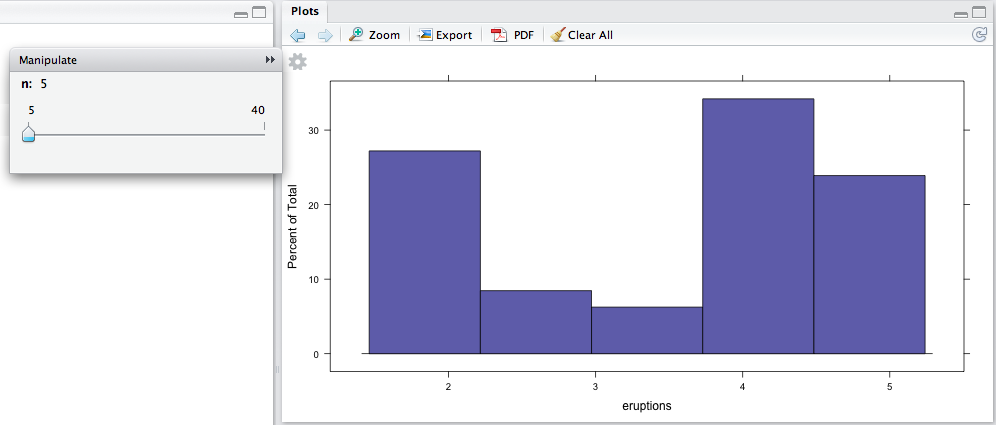
\includegraphics[width=3.8in]{images/manip-hist1.png}
\end{center}

When the slider is changed, we see a clearer view of the eruptions of Old Faithful.

\centerline{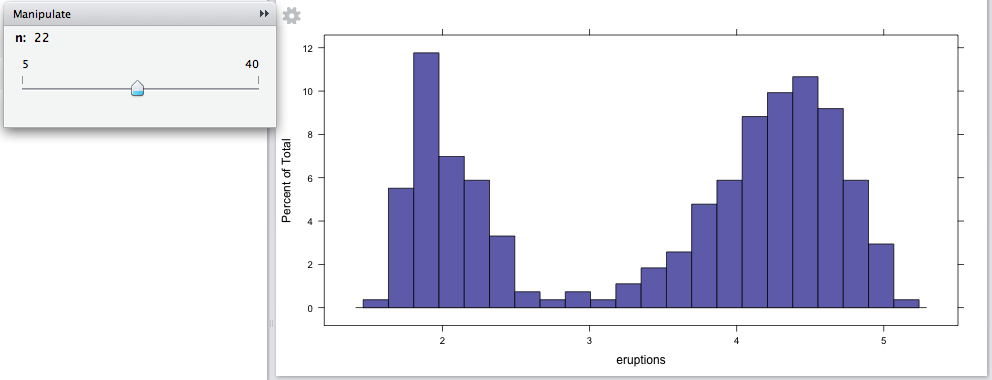
\includegraphics[width=3.8in]{images/manip-hist2.png}}



\subsection{Check Boxes}

\begin{knitrout}
\definecolor{shadecolor}{rgb}{.97, .97, .97}{\color{fgcolor}\begin{kframe}
\begin{flushleft}
\ttfamily\noindent
\hlkeyword{if}{\ }\hlkeyword{(}\hlfunctioncall{require}\hlkeyword{(}\hlsymbol{manipulate}\hlkeyword{)}\hlkeyword{)}{\ }\hlkeyword{\usebox{\hlnormalsizeboxopenbrace}}\hspace*{\fill}\\
\hlstd{}{\ }{\ }{\ }{\ }\hlfunctioncall{manipulate}\hlkeyword{(}\hlfunctioncall{xhistogram}\hlkeyword{(}\hlkeyword{\urltilda{}}\hlsymbol{age}\hlkeyword{,}{\ }\hlargument{data}{\ }\hlargument{=}{\ }\hlsymbol{HELP}\hlkeyword{,}{\ }\hlargument{n}{\ }\hlargument{=}{\ }\hlsymbol{n}\hlkeyword{,}{\ }\hlargument{density}{\ }\hlargument{=}{\ }\hlsymbol{density}\hlkeyword{)}\hlkeyword{,}{\ }\hlargument{n}{\ }\hlargument{=}{\ }\hlfunctioncall{slider}\hlkeyword{(}\hlnumber{5}\hlkeyword{,}\hspace*{\fill}\\
\hlstd{}{\ }{\ }{\ }{\ }{\ }{\ }{\ }{\ }\hlnumber{40}\hlkeyword{)}\hlkeyword{,}{\ }\hlargument{density}{\ }\hlargument{=}{\ }\hlfunctioncall{checkbox}\hlkeyword{(}\hlkeyword{)}\hlkeyword{)}\hspace*{\fill}\\
\hlstd{}\hlkeyword{\usebox{\hlnormalsizeboxclosebrace}}\mbox{}
\normalfont
\end{flushleft}
\begin{verbatim}
Loading required package: manipulate
\end{verbatim}
\begin{verbatim}
Warning message: there is no package called 'manipulate'
\end{verbatim}
\end{kframe}}
\end{knitrout}


\centerline{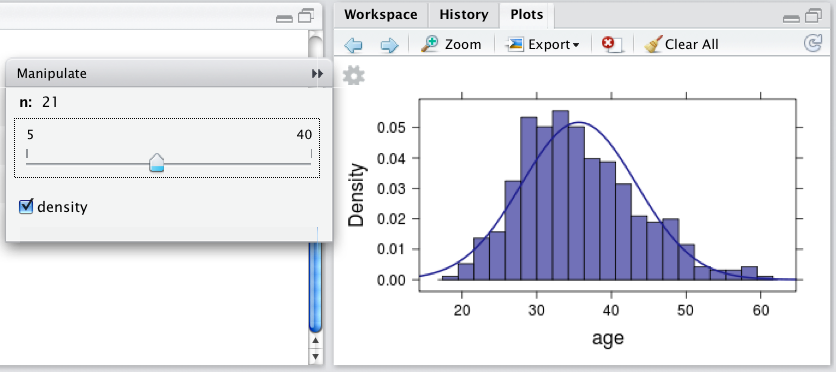
\includegraphics[width=3.8in]{images/manipulate-checkbox}}

\subsection{Drop-down Menus}

\begin{knitrout}
\definecolor{shadecolor}{rgb}{.97, .97, .97}{\color{fgcolor}\begin{kframe}
\begin{flushleft}
\ttfamily\noindent
\hlkeyword{if}{\ }\hlkeyword{(}\hlfunctioncall{require}\hlkeyword{(}\hlsymbol{manipulate}\hlkeyword{)}\hlkeyword{)}{\ }\hlkeyword{\usebox{\hlnormalsizeboxopenbrace}}\hspace*{\fill}\\
\hlstd{}{\ }{\ }{\ }{\ }\hlfunctioncall{manipulate}\hlkeyword{(}\hlfunctioncall{xhistogram}\hlkeyword{(}\hlkeyword{\urltilda{}}\hlsymbol{age}\hlkeyword{,}{\ }\hlargument{data}{\ }\hlargument{=}{\ }\hlsymbol{HELP}\hlkeyword{,}{\ }\hlargument{n}{\ }\hlargument{=}{\ }\hlsymbol{n}\hlkeyword{,}{\ }\hlargument{fit}{\ }\hlargument{=}{\ }\hlsymbol{distribution}\hlkeyword{,}{\ }\hlargument{dlwd}{\ }\hlargument{=}{\ }\hlnumber{4}\hlkeyword{)}\hlkeyword{,}\hspace*{\fill}\\
\hlstd{}{\ }{\ }{\ }{\ }{\ }{\ }{\ }{\ }\hlargument{n}{\ }\hlargument{=}{\ }\hlfunctioncall{slider}\hlkeyword{(}\hlnumber{5}\hlkeyword{,}{\ }\hlnumber{40}\hlkeyword{)}\hlkeyword{,}{\ }\hlargument{distribution}{\ }\hlargument{=}{\ }\hlfunctioncall{picker}\hlkeyword{(}\hlstring{"{}normal"{}}\hlkeyword{,}{\ }\hlstring{"{}gamma"{}}\hlkeyword{,}{\ }\hlstring{"{}exponential"{}}\hlkeyword{,}\hspace*{\fill}\\
\hlstd{}{\ }{\ }{\ }{\ }{\ }{\ }{\ }{\ }{\ }{\ }{\ }{\ }\hlstring{"{}lognormal"{}}\hlkeyword{,}{\ }\hlargument{label}{\ }\hlargument{=}{\ }\hlstring{"{}distribution"{}}\hlkeyword{)}\hlkeyword{)}\hspace*{\fill}\\
\hlstd{}\hlkeyword{\usebox{\hlnormalsizeboxclosebrace}}\mbox{}
\normalfont
\end{flushleft}
\begin{verbatim}
Loading required package: manipulate
\end{verbatim}
\begin{verbatim}
Warning message: there is no package called 'manipulate'
\end{verbatim}
\end{kframe}}
\end{knitrout}


\centerline{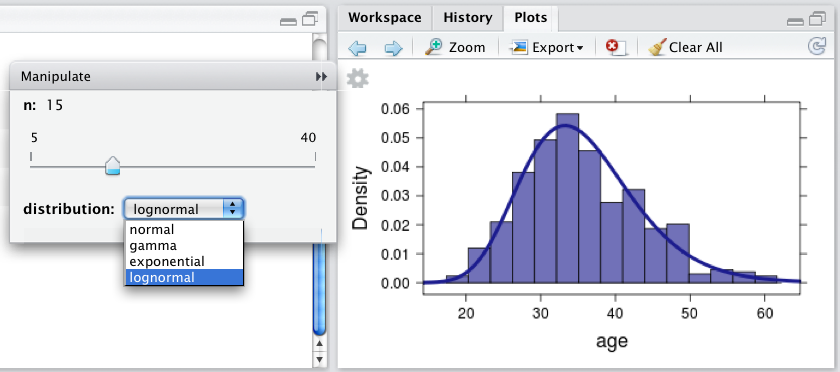
\includegraphics[width=3.8in]{images/manipulate-picker}}

\subsection{Visualizing Normal Distributions}
\begin{knitrout}
\definecolor{shadecolor}{rgb}{.97, .97, .97}{\color{fgcolor}\begin{kframe}
\begin{flushleft}
\ttfamily\noindent
\hlkeyword{if}{\ }\hlkeyword{(}\hlfunctioncall{require}\hlkeyword{(}\hlsymbol{manipulate}\hlkeyword{)}\hlkeyword{)}{\ }\hlkeyword{\usebox{\hlnormalsizeboxopenbrace}}\hspace*{\fill}\\
\hlstd{}{\ }{\ }{\ }{\ }\hlfunctioncall{manipulate}\hlkeyword{(}\hlfunctioncall{xpnorm}\hlkeyword{(}\hlsymbol{x}\hlkeyword{,}{\ }\hlnumber{500}\hlkeyword{,}{\ }\hlnumber{100}\hlkeyword{)}\hlkeyword{,}{\ }\hlargument{x}{\ }\hlargument{=}{\ }\hlfunctioncall{slider}\hlkeyword{(}\hlnumber{200}\hlkeyword{,}{\ }\hlnumber{800}\hlkeyword{)}\hlkeyword{)}\hspace*{\fill}\\
\hlstd{}\hlkeyword{\usebox{\hlnormalsizeboxclosebrace}}\mbox{}
\normalfont
\end{flushleft}
\begin{verbatim}
Loading required package: manipulate
\end{verbatim}
\begin{verbatim}
Warning message: there is no package called 'manipulate'
\end{verbatim}
\end{kframe}}
\end{knitrout}

\centerline{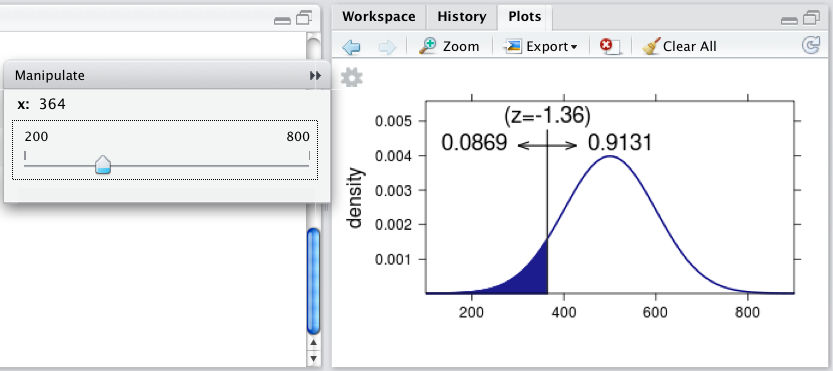
\includegraphics[width=3.8in]{images/manipulate-xpnorm}}


\begin{problem}
The following code makes a scatterplot with separate symbols for each sex.
\begin{knitrout}
\definecolor{shadecolor}{rgb}{.97, .97, .97}{\color{fgcolor}\begin{kframe}
\begin{flushleft}
\ttfamily\noindent
\hlfunctioncall{xyplot}\hlkeyword{(}\hlsymbol{cesd}{\ }\hlkeyword{\urltilda{}}{\ }\hlsymbol{age}\hlkeyword{,}{\ }\hlargument{data}{\ }\hlargument{=}{\ }\hlsymbol{HELP}\hlkeyword{,}{\ }\hlargument{groups}{\ }\hlargument{=}{\ }\hlsymbol{sex}\hlkeyword{)}\mbox{}
\normalfont
\end{flushleft}
\end{kframe}}
\end{knitrout}

Build a \pkg{manipulate} example that allows you to turn the grouping on and off with a 
checkbox.
\end{problem}

\begin{problem}
Build a \pkg{manipulate} example that uses a picker to select from a number of 
variables to make a plot for.  Here's an example with a histogram:

\medskip
\centerline{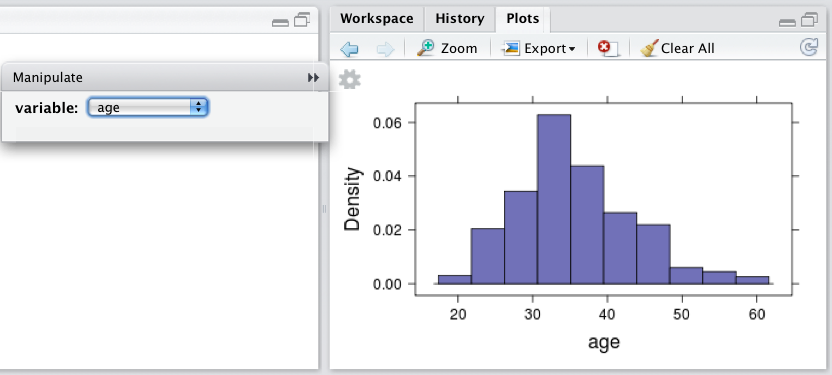
\includegraphics[width=3.8in]{images/manipulate-multihist}}
\end{problem}

\begin{problem}
Design your own  interactive demonstration idea and implement it using 
\RStudio\ \pkg{manipulate} tools.
\end{problem}

\section*{Exercises}
\shipoutProblems

